\documentclass[sigconf]{acmart}
% =============================================================================
% Template setup — participants normally do not edit this file.
% Author content belongs in main.tex; citations belong in main.bib.
% \documentclass lives in main.tex so Overleaf does not treat this file as root.
% =============================================================================

% --- Competition / non-ACM-submission friendly rights metadata -------------
\setcopyright{none}
\settopmatter{printacmref=false}
\acmConference[Kaggle Competition]{Filament Segmentation Challenge}{2026}{\href{https://www.kaggle.com/competitions/filament-segmentation-2026}{kaggle.com/competitions/filament-segmentation-2026}}
\acmBooktitle{Competition Report}
\acmDOI{}
\acmISBN{}

% --- Author guidance text --------------------------------------------------
% \guide{...} is gray italic while \guideStyletrue; omitted from the PDF if false.
% Flip the switch in main.tex after % =============================================================================
% Template setup — participants normally do not edit this file.
% Author content belongs in main.tex; citations belong in main.bib.
% \documentclass lives in main.tex so Overleaf does not treat this file as root.
% =============================================================================

% --- Competition / non-ACM-submission friendly rights metadata -------------
\setcopyright{none}
\settopmatter{printacmref=false}
\acmConference[Kaggle Competition]{Filament Segmentation Challenge}{2026}{\href{https://www.kaggle.com/competitions/filament-segmentation-2026}{kaggle.com/competitions/filament-segmentation-2026}}
\acmBooktitle{Competition Report}
\acmDOI{}
\acmISBN{}

% --- Author guidance text --------------------------------------------------
% \guide{...} is gray italic while \guideStyletrue; omitted from the PDF if false.
% Flip the switch in main.tex after % =============================================================================
% Template setup — participants normally do not edit this file.
% Author content belongs in main.tex; citations belong in main.bib.
% \documentclass lives in main.tex so Overleaf does not treat this file as root.
% =============================================================================

% --- Competition / non-ACM-submission friendly rights metadata -------------
\setcopyright{none}
\settopmatter{printacmref=false}
\acmConference[Kaggle Competition]{Filament Segmentation Challenge}{2026}{\href{https://www.kaggle.com/competitions/filament-segmentation-2026}{kaggle.com/competitions/filament-segmentation-2026}}
\acmBooktitle{Competition Report}
\acmDOI{}
\acmISBN{}

% --- Author guidance text --------------------------------------------------
% \guide{...} is gray italic while \guideStyletrue; omitted from the PDF if false.
% Flip the switch in main.tex after \input{preamble}.
%
% Do not use \guide{...} for \email{...}.
\usepackage{xcolor}
\newif\ifguideStyle
\guideStyletrue
\newcommand{\guide}[1]{%
  \ifguideStyle
    {\color{gray!65}\itshape #1}%
  \fi
}

% --- Math ------------------------------------------------------------------
% Do NOT load amssymb (or amsfonts): acmart already loads newtxmath, which
% defines the same symbols (e.g. \Bbbk) and causes a conflict on Overleaf.
% amsmath is already provided by acmart; mathtools extends it.
\usepackage{mathtools}

% --- Figures ---------------------------------------------------------------
% graphicx is already loaded by acmart
\usepackage{subcaption}

% --- Tables ----------------------------------------------------------------
% booktabs is already loaded by acmart
\usepackage{tabularx}
\usepackage{multirow}

% --- Bibliography style is set in main.tex (ACM-Reference-Format) ----------
.
%
% Do not use \guide{...} for \email{...}.
\usepackage{xcolor}
\newif\ifguideStyle
\guideStyletrue
\newcommand{\guide}[1]{%
  \ifguideStyle
    {\color{gray!65}\itshape #1}%
  \fi
}

% --- Math ------------------------------------------------------------------
% Do NOT load amssymb (or amsfonts): acmart already loads newtxmath, which
% defines the same symbols (e.g. \Bbbk) and causes a conflict on Overleaf.
% amsmath is already provided by acmart; mathtools extends it.
\usepackage{mathtools}

% --- Figures ---------------------------------------------------------------
% graphicx is already loaded by acmart
\usepackage{subcaption}

% --- Tables ----------------------------------------------------------------
% booktabs is already loaded by acmart
\usepackage{tabularx}
\usepackage{multirow}

% --- Bibliography style is set in main.tex (ACM-Reference-Format) ----------
.
%
% Do not use \guide{...} for \email{...}.
\usepackage{xcolor}
\newif\ifguideStyle
\guideStyletrue
\newcommand{\guide}[1]{%
  \ifguideStyle
    {\color{gray!65}\itshape #1}%
  \fi
}

% --- Math ------------------------------------------------------------------
% Do NOT load amssymb (or amsfonts): acmart already loads newtxmath, which
% defines the same symbols (e.g. \Bbbk) and causes a conflict on Overleaf.
% amsmath is already provided by acmart; mathtools extends it.
\usepackage{mathtools}

% --- Figures ---------------------------------------------------------------
% graphicx is already loaded by acmart
\usepackage{subcaption}

% --- Tables ----------------------------------------------------------------
% booktabs is already loaded by acmart
\usepackage{tabularx}
\usepackage{multirow}

% --- Bibliography style is set in main.tex (ACM-Reference-Format) ----------

\guideStylefalse
\setlength{\emergencystretch}{3em}

\begin{document}
\title{Solar Filament Instance Segmentation with Mask-Guided Refinement and Cross-View Voting}
\subtitle{A Solution to the Solar Filament Segmentation Challenge 2026}
\author{Rahul Singh}
\email{rahulsingh.rs.career@gmail.com}

\begin{abstract}
This report describes our solution to the Solar Filament Segmentation Challenge~2026, a Kaggle competition on automatic segmentation of solar filaments in GONG H-$\alpha$ observations. YOLO11s-seg proposes instances and a mask-guided U-Net refines each proposal at crop scale. A horizontally flipped view corroborates isolated detections, and a third, higher-resolution view contributes to a pixel vote on matched instances. On a day-separated validation split of 146 physical images and 234 annotation records, the final recipe achieves 0.463374 pooled panoptic quality (PQ), with 994 true positives, 426 false positives, and 528 false negatives. Kaggle displayed public PQ of 0.37 for the submitted CSV.
\end{abstract}
\maketitle

\section{Introduction}
This report goes over the details of our submitted solution to the Solar Filament Segmentation Challenge~2026 \cite{filament-segmentation-2026}. The challenge, launched on July~10,~2026, is organized by the Earth-Space AI Research (ESAIR) Lab\footnote{\href{https://www.esairlab.com/home}{www.esairlab.com/}}. This challenge utilizes the MAGFiLO dataset for evaluation of the segmentation algorithms \cite{ahmadzadeh2024dataset}. The pipeline uses full-disk context to propose instances and a separate crop-scale model to recover boundaries. The final step uses agreement across detector views to adjust an instance without taking pixels from its neighbors.

\section{Methodology}

\subsection{Data and detector}
The labeled split contains 707 physical images and 1,154 annotation records. Whole observation days are assigned to training (561 images, 920 records) or validation (146 images, 234 records and 1,522 target masks). Multiple annotations of an image remain independent records in the same split. The detector trains on one-class polygon labels and evaluation uses original raster masks.

We fine-tune COCO-initialized YOLO11s-seg using Ultralytics 8.3.85~\cite{yolo11}. Training uses 2048-pixel input, AdamW, physical batch size 1, nominal batch size 8, and 30 epochs. The epoch-26 checkpoint is selected by local validation PQ and frozen. Inference uses detector NMS IoU 0.70, at most 100 proposals, and mask restoration to native coordinates. Only the supplied H-$\alpha$ image is required at inference.

\begin{figure}[t]
\centering
\fbox{\begin{minipage}{0.94\columnwidth}
\centering
Native $2048\times2048$ H-$\alpha$ observation\\[2pt]
$\downarrow$\\
Original 2048 \quad|\quad Flipped 2048 \quad|\quad Original 2560\\
YOLO11s-seg per view, then align to native coordinates\\[2pt]
$\downarrow$\\
Grayscale and coarse-mask crops $\rightarrow$ shared U-Net\\[2pt]
$\downarrow$\\
Clean original instances and admit isolated mirror detections\\[2pt]
$\downarrow$\\
Match against flipped and 2560 masks, then vote on pixels\\[2pt]
$\downarrow$\\
Check disjoint masks $\rightarrow$ compressed COCO RLE CSV
\end{minipage}}
\caption{The three-view inference pipeline. All views use the same detector and refiner weights.}
\Description{A flow diagram from the solar observation through three aligned detector views, shared mask-guided refinement, mirror admissions, boundary voting, and disjoint mask export.}
\end{figure}

\subsection{Mask-guided refinement and cleanup}
We pad each proposal's mask bounds by 32 pixels, clip to the image, and map the grayscale crop and coarse mask to a $512\times512$ canvas. A randomly initialized, two-channel ResNet34 U-Net with GroupNorm receives one coarse mask as an instance prompt~\cite{resnet,unet}. We train with valid-pixel BCE and soft Dice over 4,589 eligible proposal--annotation pairs, batch size 2, and AdamW at $3\times10^{-4}$. Each completed pass visits all pairs. The planned ten-pass schedule completed eight passes before stopping during pass nine. We use the saved pass-six checkpoint.

At inference we map mask probabilities back to native coordinates and threshold at 0.55, with the coarse mask as fallback for an empty result. The original view admits proposals at confidence 0.20 for cleanup. Image-supported restoration and candidate reranking precede duplicate suppression. Geometry checks govern fragment grouping before shared pixels are assigned. Final filters remove tiny remnants and weak outputs without coarse or competing-proposal support.

\subsection{Mirror admissions and boundary voting}
We run the flipped view at confidence 0.15 and reverse the flip on coarse masks before refinement against the original grayscale image. An original candidate at confidence 0.18 or above can be appended when it is a mutual best match with a flipped candidate, with coarse IoU at least 0.45, refined IoU at least 0.50, and mean confidence at least 0.24. A flipped candidate at confidence 0.35 or above can also be appended. Each addition must be disjoint from accepted instances.

The third detector view uses the unflipped image at 2560-pixel input and confidence 0.18. The flipped and 2560 masks considered for voting have confidence at least 0.20. Each final mask must be a mutual best match to a candidate in each auxiliary view, and all three pairwise IoUs must be at least 0.65. A pixel survives if at least two of the three masks include it. The original mask is retained if the vote would overlap another instance.

\section{Evaluation}
We follow the organizer's self-evaluation convention~\cite{selfeval}. A match requires mask IoU greater than 0.50. The same prediction set is evaluated separately against each annotation record. We pool qualifying IoUs and TP, FP, and FN before computing PQ.

\begin{table}[h]
\centering
\caption{Local validation results on 234 annotation records.}
\begin{tabular}{lrrrr}
\toprule
Recipe & PQ & TP & FP & FN\\
\midrule
Original view & 0.458323 & 976 & 413 & 546\\
Mirror admissions & 0.459652 & 990 & 430 & 532\\
Vote, no flipped view & 0.459030 & 976 & 413 & 546\\
Three-view vote & \textbf{0.463374} & 994 & 426 & 528\\
Vote plus isolated admissions & 0.465434 & 1013 & 446 & 509\\
\bottomrule
\end{tabular}
\end{table}

Voting gains seven annotation matches and loses three relative to mirror admissions. It keeps the same 928 physical masks and improves local PQ for each of the six observatory groups. A paired bootstrap over 132 observation days gives a descriptive 95\% interval of $[0.00169, 0.00580]$ for the change in PQ. The validation set was reused in development, so the interval does not establish improvement on new data. Both three-view submissions displayed public Kaggle PQ of 0.37, with the plain vote listed higher. Unrounded and private scores are unavailable. We select the plain vote.

\begin{figure*}[t]
\centering
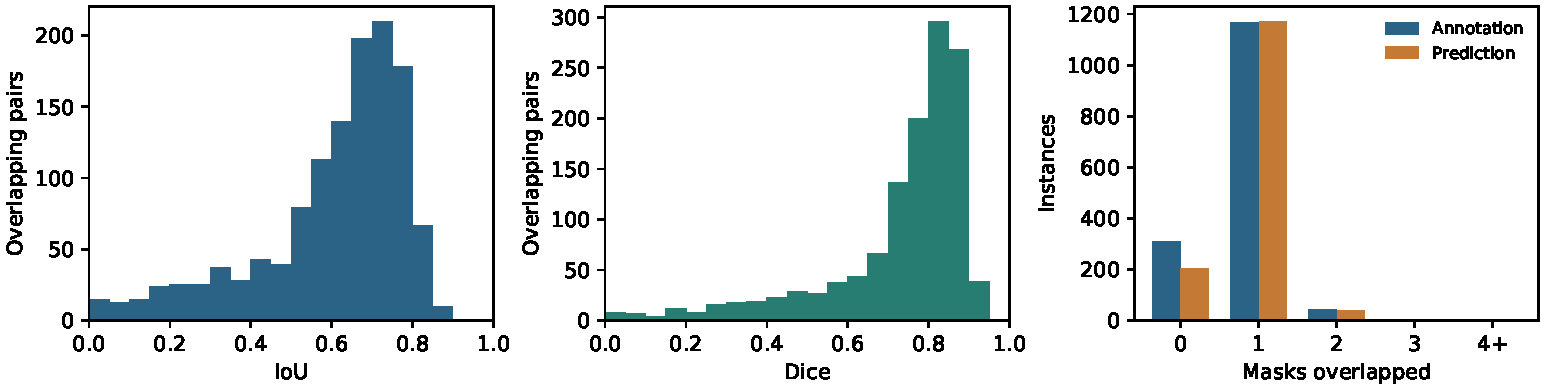
\includegraphics[width=\textwidth]{figures/validation-metrics.pdf}
\caption{Validation IoU and Dice for all nonzero prediction--annotation pairs, and the number of overlapping masks per instance at IoU greater than zero.}
\label{fig:metrics}
\Description{Histograms of positive pairwise IoU and Dice and a grouped bar chart of geometric overlap counts.}
\end{figure*}

Across 1,260 overlapping pairs, median IoU is 0.659 and median Dice is 0.795. Forty-five annotation instances overlap multiple predicted masks, and 42 prediction instances overlap multiple annotated masks when counted per record. These are geometric overlap counts. They include partial overlaps and cases where annotators disagree about grouping.

\begin{figure*}[t]
\centering
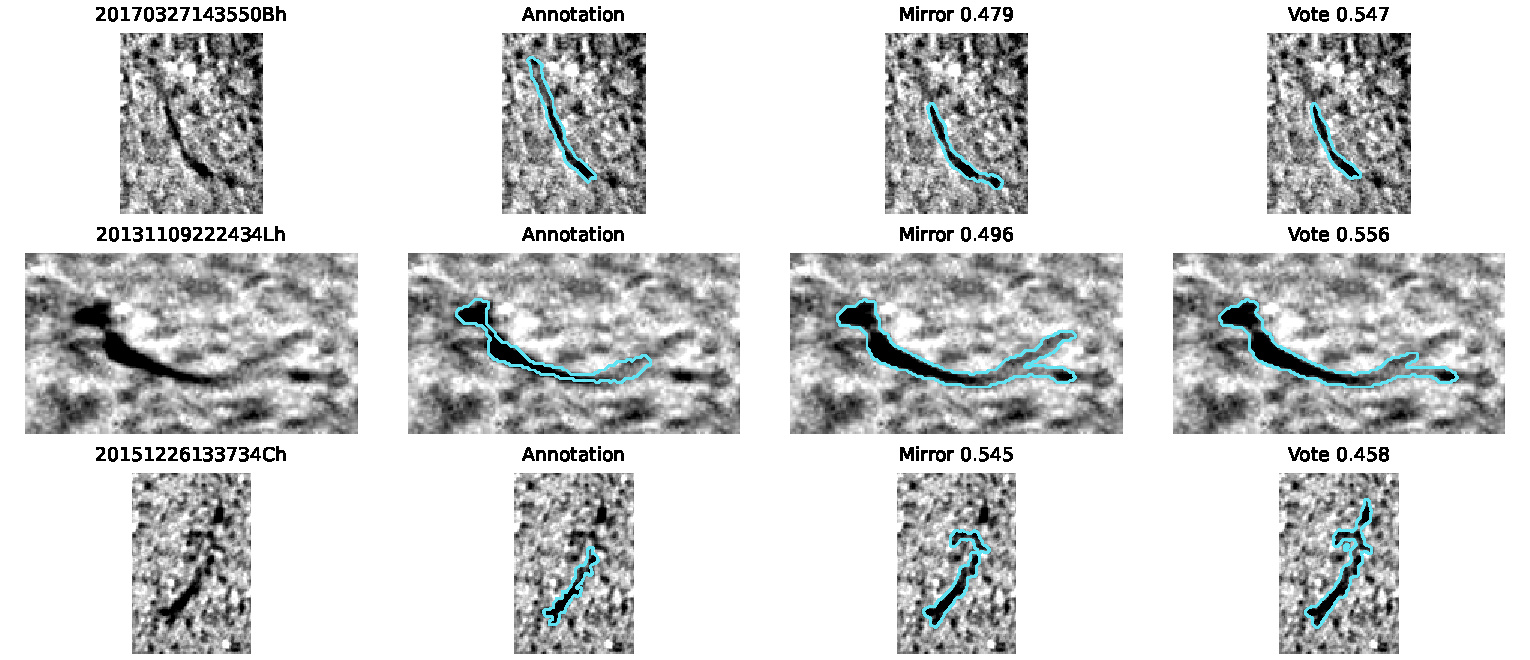
\includegraphics[width=\textwidth]{figures/boundary-examples.pdf}
\caption{Validation crops showing two recovered matches and one lost match. The overlay traces one mask per panel. Values are IoU against the selected annotation.}
\label{fig:cases}
\Description{Three rows of grayscale solar crops compare one reference contour, the mirrored pipeline, and the final vote.}
\end{figure*}

Of 528 missed annotations, 187 had at least one qualifying refined candidate at confidence 0.20 or above among the cached views. A further 122 had no overlapping candidate in those caches. The first group motivates better instance selection. The second suggests improving proposal coverage. Figure~\ref{fig:cases} shows how voting can correct a boundary or remove a previously adequate match.

\subsection{Efficiency and reproduction}
On an RTX 3060 Ti with PyTorch 2.6.0 and CUDA 12.6, a warm pass over the 146 validation images averaged 5.09 seconds per image for inference and cleanup, versus 4.08 seconds for the mirrored recipe. Including CSV writing and verification, voting took 13.6 minutes, excluding model loading. This is a single measured run with shared computation for the timing comparison.

The supplied notebook calls the same inference code as the CLI. Pinned dependencies and SHA-256 checks identify the software and checkpoints. The exported CSV processed all 180 test images and contains 1,187 unique, nonempty, disjoint masks. Each uses canonical compressed COCO RLE at native resolution. Three images produced no instances. Code and checkpoints accompany the submission at \url{https://github.com/rahulcomet/solar-filament-segmentation}.

\clearpage
\section{Acknowledgment}
The organization of the Filament Segmentation Challenge 2026 is partially supported by the U.S. National Science Foundation (NSF) under Grant No. 2209912 and 2433781, directorate for Computer and Information Science and Engineering (CSE), and Office of Advanced Cyberinfrastructure (OAC), and Grant No. 2511630, AST Division Of Astronomical Sciences and MPS Directorate for Mathematical and Physical Sciences.

The Filament Segmentation Challenge 2026 is sponsored by the U.S. National Science Foundation (NSF) National Solar Observatory (NSO).

This work utilizes GONG data obtained by the NSO Integrated Synoptic Program, managed by the National Solar Observatory, which is operated by the Association of Universities for Research in Astronomy (AURA), Inc. under a cooperative agreement with the National Science Foundation and with contribution from the National Aeronautics and Space Administration. The GONG network of instruments is hosted by the Big Bear Solar Observatory, High Altitude Observatory, Learmonth Solar Observatory, Udaipur Solar Observatory, Instituto de Astrof\'isica de Canarias, and Cerro Tololo Interamerican Observatory.

\bibliographystyle{ACM-Reference-Format}
\bibliography{main}
\end{document}
